\section{On Job and Suffering}

\begin{quotex}
There never was, and never will be a place on earth free from sorrows. The only sorrow-less place possible is in the heart, when the Lord is present there.
\flright{\textsc{St Nikon of Optina}}
\end{quotex}


\subsection*{I. Introduction}

\begin{wrapfigure}{rt}{.4\textwidth}
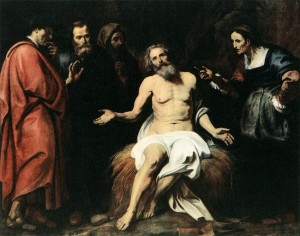
\includegraphics[scale=.45]{a20131006OnJobandSuffering-img001.jpg} 
\end{wrapfigure}

Job in the Bible is a powerful text. It can be seen in many lights, and render different interpretation. Most of the medieval commentators of the book have seen Job as the enduring ideal; he lost everything, yet in the end, he still sides with God. Through those readings, we can also understand other insights that lead to different questions about God, sorrow and suffering.

First we must understand that Job challenge God. If we think that Job is passive toward God, then we lose perspective and understanding of his plea. This challenge is formulated toward what happens to him; but also what happens everywhere.

The question of Job is therefore not ”Why me?”, but rather ”Why us God?”. He speaks to Him as a fallen Adam, representing the whole of human race that demands answer on suffering: why is it that God let the world be ”imperfect” and why doesn't he act upon it? Is He not all-powerful? The theodicy therefore becomes a question of cosmodicy.

As a side note, the focus should not be put between Satan and God, but rather between human and humans, and in the end, between God and Adam. Satan here is to be taken as an older form of the character, and represent an accusation toward Job (the word Satan can be interpreted as ”the accusator”). It is not about a cosmic battle between God and Satan, as this would be futile in the conclusion of God answer to Job (more on it later). The focus is on God himself: it is theocentric. In the same vein, if there is some difference and contradiction with other books of the Bible such as Genesis, we must not see them as being unrelated: the author of Job wrote with Genesis in mind, and he gave us a complementary observation that leads to questions and insights on the world. Also, I will by no means elucidate the book for ever and ever. Hermeneutics and the understanding of God cannot be depleted in formal texts and words like this. Also, Job is a book rich in meanings that demands also subjective understanding.

In Latin, the word for suffering is linked deeply with the action of bearing, or sustaining. That suffering is associated with evil. In French this is even easier to understand ”J'ai \emph{mal}”, literally translated as ”I have evil” (which means ”\emph{I have pain”}). In the case of Job, this suffering is ”unjustified”, and is not a moral suffering, neither a ”natural” suffering; nor is it just physical or psychic : he also suffers because God doesn't answer him. He has in himself pure suffering, on every level of his being. The question in Job is not only around suffering, but much more about language, and how we can speak of/about God.

Also we must keep in mind that Job faith is disinterested. He doesn't ask for more riches, for resurrection, for anything but God Himself. It is also stated that he is a stranger, a non-Israelite, yet he still believes. It is a free faith.

\subsection*{II. On Job}

The ``friends” of Job answer to him using different approach to evil and suffering. Some uses collective retribution, individual retribution, immanent justice, radical indignity of man, divine pedagogy, etc. Most of them sound like purely exoteric, often even liberalist or modern by standard. Job himself doesn't revolt so much against suffering in the dialogue, but rather against the speech of his friends; they are speaking lies. Job refuses a theology that is not anchored in experience and into which truth is grafted. Truth must be appropriated.

Of course, the character of Job is a rebel, but a ``just rebel” in the sense that he doesn't see fit to negate God, neither diminish Him: he wants to speak to Him, to understand. To Job, there is no ``interested faith” in resurrection or supra-terrestrial retribution: he prays to God in gratuity and disinterest; therefore Satan lost his bet.

The answer of God seems to cause problem to most readers; but in truth, this answer is all that was needed. God tell Job that he was right to revolt; because he continued to believe. Job asked for God to see him, and He did. He accuses the ``friends” of Job of speaking ill: their ``ethics” are a source of immorality because morality cannot think theologically suffering, less so think God. God refuses to let Himself be caged in the logicality of morality and retribution. In doing so, God sets himself free of an anthropocentric soteriology. God recognize existence of ``evil suffering” (that is, suffering without logical explanation that derives from chaos and non-being) that can be fought against (see the teachings on Behemoth and Leviathan). God shows Job his temporal finitude, his spatial finitude and his ignorance. God shows that His will and Goodness is not for human only, but for the whole of Creation (Job 38, 26 compare GN 5, 10; there is no necessity in God's Love). God, by showing His gratuitous creative Will and Love, takes the fight directly beyond anthropocentric views. And that is the whole of God answer to suffering even if he does not answer it ‘‘directly’’: suffering and evil will always be difficult to ``bear”, to ``support” (latin ``\emph{suffere}”) if one center his view on Man as man. But if he does it as Creation (Adam) on God, everything changes. Humanity is not the center of God, He is the center of All; therefore, Job, as man, is not the measure of things. Man is a stranger in a strange land, God rejoice of Himself and Creation without him: Job cannot judge creation from an anthropocentric perspective (that is, a finite and non-static point of view). Only God can be the Final Judge. He asks Job to go beyond anthropocentric existentialism. Job finally understand his finite nature on earth, and by this dialogue with God, retake his dignity of Adam the Fallen that wants to be reunited with Him.

\begin{quotex}
Man is not the centre. God does not exist for the sake of man. Man does not exist for his own sake.
\flright{\textsc{C.S. Lewis}}
\end{quotex}

On Behemoth and Leviathan: God makes us remember that where it is chaotic, it needs not be Chaos. In other words, nature and animals as they are represent a form of chaos (see ancient kings hunting animals through their kingdom to make it safer, more ``orderly”). Yet this chaos is not to man's command, it is only to God. Evil is fought upon, but never totally destroyed; if chaos was to be destroyed, evil with it, there would be no more liberty, no more free will. The very existence of evil and chaos gives man the choice between them both, and ultimately to transcend them both to regain access to God directly. Liberty exists in the cosmos so that we can use free-will to (Love) rejoice in God. On the other hand, if there would be only Chaos, then nothing could be. Everything would be pure materiality without form. In other words, God do fight evil: he constrains it and rule over it so that there is a balance that permits us to love and serve Him. He is therefore the first of those who fight Evil and Chaos. And we, as Adam, must share this fight in the ordering of the cosmos, the society, the family, the body and most importantly, our mind and being. We participate in the order of God by being orderly and constraining chaos within ourselves.

\begin{quotex}
In the same line of thought, we will say thus : it is absurd to condemn the world of its imperfections while admitting the existence of the same world, and ask ourselves why injustice and suffering exist, because if one says ``exist”, one says ``to be separated from God”, therefore, from Perfection; who says ``effect”, says ``distance from the Cause”, in such that Existence implies inherently imperfection. A sorrowful separation, for exemple, already exist in the distinction of the pure spatiality of the body; then it is illogical to admit the spatial distinction while being astonished by a moral separation. The roots of all evil, we repeat, is the ontological distance between the world and God, that which cannot not exist, God being infinite; this distance echoes throughout all of Existence.

\flright{\textsc{Schuon}, \textit{Les stations de la sagesse}}
\end{quotex}


\subsection*{III. Conclusion}

As such, Job represents the perfect believer: he serves without having seen or received, and serves with a disinterested will. Even after speaking with God, there is no mention of seeing directly God or his energies; rather he saw Creation under a new eye. The truth of Creation is the truth of foundation (Temple of Jerusalem) and the truth of Christ. God is present through his creation like he is through His Temple or His Son. God is the angular stone of the Cosmos. God gives Himself to see everywhere: it is up to us to see it. Therefore the world is not a dark illusion, but a grand theophony in which God reveal Himself in Himself by Himself. In being totally transcendent, yet present in the immanence, there is a rejection of dualism and pantheism (non-dualism). God reveal Himself in a sacramental character (as Christ reveal Himself in the Eucharist) through creation; there is an earthly symbolism in the cosmos that allude to supra-terrestrial symbols. What are symbols therefore? Unification of the Divine and the Human. God and Adam. Therefore Creation is, as Philo, Eckhart, St Bernard and St Thomas Aquinas said, an open book for us to understand and behold the Creator.

There is some arguments against God, for God, through God: but never without God. Job is there to remember us that we can live and think everything through God; in other words, we need not to stop believing or desire knowing God because of contingent acts (like suffering). There is no possible atheism; the problem is not with God, but with Man. There is no need to condemn man for suffering, nor is there reason to stop believing in God. In light of this, we could give back the title of All-Powerful to God, only we have to see this in another way: God is Powerful in the Aristotelian sense of power, that is, He is not in act while in power. Why? Because he does indeed act upon evil, but not in an ”all” way, or He would destroy free-will with evil (Genesis 18:23-33).

World is therefore the Grail of God. He pours Himself into it. We can try to represent this constant revelation and order (see above) through art: art as the formal revelation of this truth. Therefore Man is to be understood as a divine animal who reintroduce the Absolute in the Relative, that participate in Him.

Knowing all this, we can understand better sin. Sin is not an objective concept, or it would relate to the Absolute. It is purely subjective, because it doesn't exist in God. When we sin, we fail to reach God. When we are washed of sin in Christ, we are washed of subjectivity and participate in the absolute Godhead. Sin is the separation from the unity of God as death is the separation from the body.

 

We thank Jean-Jacques Lavoie for insights on this powerful text.

\flrightit{Posted on 2013-10-06 by David}
